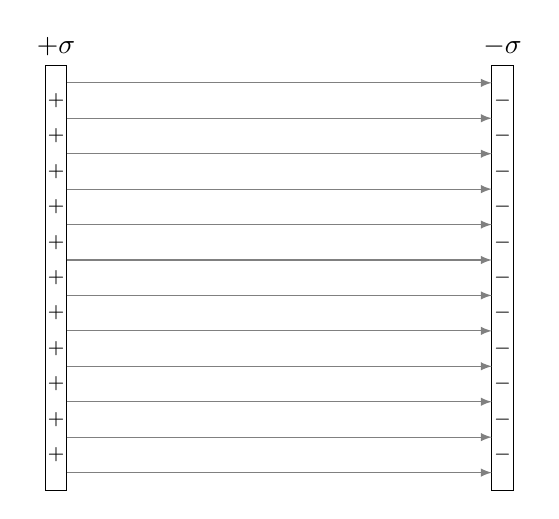
\begin{tikzpicture}[scale=0.9]
    \draw(-3.3,3) rectangle (-3.0,-3);
    \draw(3.3,3) rectangle (3.0,-3);
    \foreach \i in{2.5,2.0,...,-2.5}
    {
        \node at (-3.15,\i) {\scriptsize $+$};
        \node at (+3.15,\i) {\scriptsize $-$};
    }
    \node[above] at(-3.15,3) {$+\sigma$};
    \node[above] at(+3.15,3) {$-\sigma$};
    \foreach \i in {2.75,2.25,...,-2.75}
    {
        \draw[-latex,gray] (-3,\i)--(3,\i);
    }
\end{tikzpicture}
